\documentclass[letterpaper, 11 pt, onecolumn]{ieeeconf}  % Comment this line out if you need a4paper

%\documentclass[a4paper, 10pt, conference]{ieeeconf}      % Use this line for a4 paper

\IEEEoverridecommandlockouts                              % This command is only needed if 
                                                          % you want to use the \thanks command
\pdfminorversion=4
\overrideIEEEmargins                                      % Needed to meet printer requirements.

% See the \addtolength command later in the file to balance the column lengths
% on the last page of the document

\makeatletter
\let\proof\@undefined
\let\endproof\@undefined
\makeatother
% The following packages can be found on http:\\www.ctan.org
%\usepackage{graphics} % for pdf, bitmapped graphics files
%\usepackage{epsfig} % for postscript graphics files
%\usepackage{mathptmx} % assumes new font selection scheme installed
%\usepackage{times} % assumes new font selection scheme installed
\usepackage[pdftex]{graphicx}
\usepackage{epstopdf}
\usepackage{amsmath} % assumes amsmath package installed
\usepackage{amssymb}  % assumes amsmath package installed
\usepackage{amsthm}
\usepackage{cite}

% *** SUBFIGURE PACKAGES ***
%\ifCLASSOPTIONcompsoc
% \usepackage[caption=false,font=normalsize,labelfont=sf,textfont=sf]{subfig}
%\else
  \usepackage[caption=false,font=footnotesize]{subfig}
%\fi
% subfig.sty, written by Steven Douglas Cochran, is the modern replacement
% for subfigure.sty, the latter of which is no longer maintained and is
% incompatible with some LaTeX packages including fixltx2e. However,
% subfig.sty requires and automatically loads Axel Sommerfeldt's caption.sty
% which will override IEEEtran.cls' handling of captions and this will result
% in non-IEEE style figure/table captions. To prevent this problem, be sure
% and invoke subfig.sty's "caption=false" package option (available since
% subfig.sty version 1.3, 2005/06/28) as this is will preserve IEEEtran.cls
% handling of captions.
% Note that the Computer Society format requires a larger sans serif font
% than the serif footnote size font used in traditional IEEE formatting
% and thus the need to invoke different subfig.sty package options depending
% on whether compsoc mode has been enabled.
%
% The latest version and documentation of subfig.sty can be obtained at:
% http://www.ctan.org/tex-archive/macros/latex/contrib/subfig/

\newtheorem{theorem}{Theorem}
\theoremstyle{definition}
\newtheorem{definition}{Definition}
\newtheorem{proposition}{Proposition}
\newtheorem{corollary}{Corollary}
\newtheorem{prob}{Problem}
 \renewcommand{\QED}{\QEDopen}

\newcommand{\halfL}{\sigma}


\title{\LARGE \bf
Notes on Variational Obstacle Path Planning using the Weighted $L_p$ Norm
}


\author{Nak-seung P. Hyun$^{1}$, Leonardo Colombo$^{2}$ % <-this % stops a space
%\thanks{*This work was supported by NSF grant CMMI$-1400256$.}% <-this % stops a space
\thanks{1. N. P. Hyun is with the School of Electrical and Computer Engineering,
Georgia Institute of Technology, Atlanta, GA, USA. 2. L. Colombo is with ACCESS Linneaus Center, Department of Automatic
Control, School of Electrical Engineering, KTH Royal Institute
ofTechnology, Osquldas vag 10, 10044, Stockholm, Sweden.
Email: $1.$ nhyun3@gatech.edu, $2.$ colombo2@kth.se}%
}

\begin{document}



\maketitle
\thispagestyle{empty}
\pagestyle{empty}


%%%%%%%%%%%%%%%%%%%%%%%%%%%%%%%%%%%%%%%%%%%%%%%%%%%%%%%%%%%%%%%%%%%%%%%%%%%%%%%%
\begin{abstract}
In this technical note, an optimal safe path planning for unicycle robot in the planar space is considered using the weighted $L_p$ norm. The nominal trajectory minimizing the cost function composed with curvature, velocity and circular obstacle potential in \cite{Colombo2017cdc} is used to generate the safe trajectory. In this paper, the geometry of the obstacle is generalized to ellipsoidal and rectangular by using the weighted $L_p$ norm shown in \cite{Hyun2017Lp}. The nominal trajectory of the robot is then formulated with the boundary value problem (BVP) of twelve dimensional ordinary differential equation. BVP is then solved numerically by using the collocation method instead of the shooting method. 
\end{abstract}

%%%%%%%%%%%%%%%%%%%%%%%%%%%%%%%%%%%%%%%%%%%%%%%%%%%%%%%%%%%%%%%%%%%%%%%%%%%%%%%%
\section{Obstacle potential using weighted $L_p$ norm}

Suppose that $x\in\mathbb{R}^n$ being positive means element-wise positive, then the weighted $L_p$ norm is defined with the positive vector $\halfL>0$ for some $\halfL\in\mathbb{R}^n$. 
\begin{definition}[Weighted $L_p$ norm]
\label{def:weighted_Lp}
Let $\halfL \in \mathbb{R}^n$ be a positive vector, and $0 < p < \infty$, 
then $||\cdot||_{\halfL, p}:\mathbb{R}^n\to\mathbb{R}_{\geq 0}$ is the
$\halfL$-weighted $L_p$ norm such that
\begin{equation*}
  ||x||_{(\halfL,p)} := \left(\sum_{i=1}^n 
         ({|x_i|}/{\halfL_i})^p\right)^{\frac{1}{p}},
\end{equation*} 
\end{definition}
The one level set of the weighted $L_p$ approaches to the rectangle with half lengths $\halfL$ in $\mathbb{R}^2$ as $p$ goes to infinity. In addition, if $p=2$, then the one level set is equal to ellipse. More detailed boundary design of the obstacle with different $p$ values can be found in \cite{Hyun2017Lp}. 

In this paper, rectangular obstacles are considered and approximated by the level set of weighted $L_p$ norm for some $p$ and $\halfL$. Remark that the circular or elliptical obstacle can be modeled simply by choosing appropriate $p$ an $\halfL$ without sacrificing anything. 

Suppose that $g_o\in SE(2)$ represents the obstacle frame relative to some world frame, and let $g_o= [x_o, y_o, \theta_o]$. The shape of the robot is defined by the half lengths $\halfL_o$ and some even $p_o$. Without loss of generality we define $g_o:SE(2)\to SE(2)$ as a transformation from the obstacle frame to world frame, and $g_o^{-1}$ does the inverse transformation. 

In the planar space, the obstacle potential, $V:\mathbb{R}^2\to\mathbb{R}^2$ is now defined as 
\begin{equation}
V(q):=\frac{\tau}{||g_o^{-1}(q)||_{(\halfL_o,p_o)}^{p_o}-1}
\end{equation} 
for $q\in\mathbb{R}^2$.

The potential for the circular obstacle with radius $r>0$ in \cite{Colombo2017cdc} will be a special case when half lengths are chosen by $\halfL=[r,r]$ and $p=2$. 

\section{Optimal path plannign} 
The above potential is then used to derive the necessary condition for the optimization problem,
\begin{equation}
\min_{g(\cdot)\in SE(2)} \int_{0}^T ||\ddot{g}||^2+\sigma||\dot{g}||^2+V(Pos(g))
\end{equation}
with $g(t)=[x(t), y(t), \theta(t)]$ for $t\in [0,T]$ represents the trajectory of the point mass unicycle and $Pos(g):=[x,y]$. The initial and final configuration and the linear and angular velocities of the robot  are constraints is given by 
\begin{eqnarray}
\label{eqn:bv_initial_config}
g(0)=g_i=[x_0, y_0, \theta_0]
\\
\label{eqn:bv_final_config}
g(T)=g_f=[x_f, y_f, \theta_f]
\\
\label{eqn:bv_initial_speed}
\dot{g}(0)=\dot{g}_i=[x^\prime_0, y^\prime_0, \theta^\prime_0]
\\
\label{eqn:bv_final_speed}
\dot{g}(T)=\dot{g}_f=[x^\prime_f, y^\prime_f, \theta^\prime_f]
\end{eqnarray} 
In addition, the nonholonomic constraint for the unicycle is given by
\begin{equation}
\label{eqn:nonholonomic}
\dot{x}\sin(\theta)-\dot{y}\cos(\theta)=0.
\end{equation}

Similar to \cite{Colombo2017cdc}, the nominal trajectory can be achieved by solving the following BVP.
\begin{eqnarray}
\label{eqn:dyn1}
\theta^{(4)}(t) &=& \sigma\theta^{(2)}(t)-1/J\lambda(t)(\dot{x}(t)\cos(\theta(t))+\dot{y}(t)\sin(\theta(t)))
\\
\label{eqn:dyn2}
x^{(4)}(t) &=& \sigma x^{(2)}(t)+\frac{\tau p_or_x(t)^{p_o-1}}{\halfL_o(1)^{p_o}}\frac{1}{m(||g_o^{-1}(Pos(g))||_{(\halfL_o,p_o)}^{p_o}-1)^2}+\frac{1}{m}(\dot{\lambda}(t)\sin(\theta(t))+\lambda(t)\dot{\theta}(t)\cos(\theta(t)))
\\
\label{eqn:dyn3}
y^{(4)}(t) &=& \sigma y^{(2)}(t)+\frac{\tau p_or_y(t)^{p_o-1}}{\halfL_o(2)^{p_o}}\frac{1}{m(||g_o^{-1}(Pos(g))||_{(\halfL_o,p_o)}^{p_o}-1)^2}+\frac{1}{m}(-\dot{\lambda}(t)\cos(\theta(t))+\lambda(t)\dot{\theta}(t)\sin(\theta(t)))
\end{eqnarray}
where $[r_x(t),r_y(t)]:=g_o^{-1}(Pos(g))$. 

\section{Solution to BVP}

In this section, the above BVP is solved by using the collocation method. The $g(t)$ is approximated by piecewise B-spline polynomials, and the above 12 boundary constraints, 3 dynamics constraints, and 1 nonholonomic constraint is given for the constraints on the coefficients of B-splines. By sampling on the collocation time for each B-splines, the BVP is convereted to the NLP problem with an auxiliary cost function, which we choose as
\begin{equation}
J(X) = \int_0^T (\dot{x}\sin(\theta)-\dot{y}\cos(\theta))^2
\end{equation}
where $X$ represents the free coefficients to optimize. 


\subsection{Simulation}

The initial and final configuration and velocities are given as
\begin{eqnarray}
g(0)=[-3, 0, \pi/4]
\\
g(T)=[3, 0.5, 0]
\\
\dot{g}(0)=[0, 0, 0]
\\
\dot{g}(T)=[0, 0, 0]
\end{eqnarray}
The obstacle $g_o=[0,0,0]$ where the center is located at $(0,0)$ and its orientation is aligned to the world frame.
\begin{figure*}[t!]
  \captionsetup[subfigure]{}
  \centering
  \hfill
  %PATRICK: PLEASE CREATE THE IDEAL CASE.
  \subfloat[ $\halfL_o= (2,1)$ and $p=6$]
    {{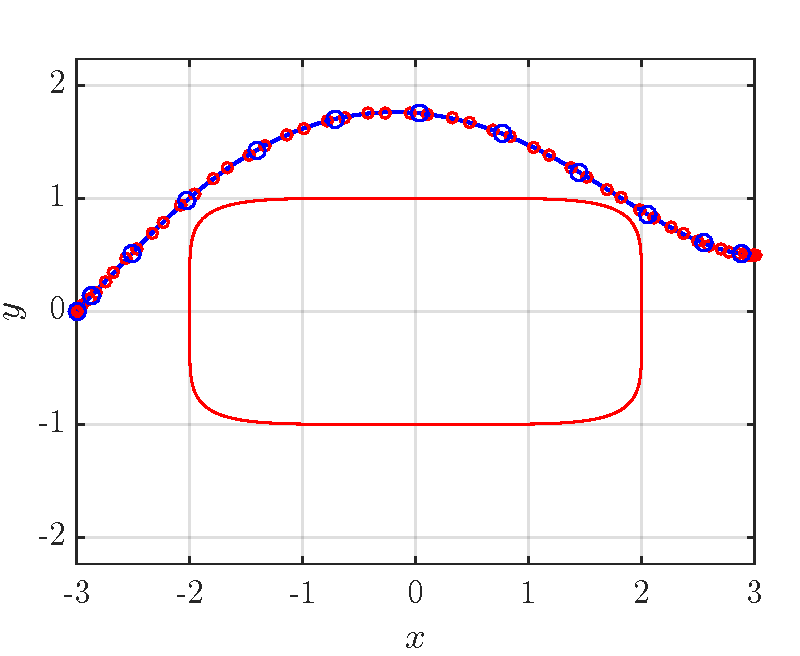
\includegraphics[width=0.33\textwidth, clip=true,trim=0.15in 0in 0.55in 0.45in]{VariationalPathPlan_Rec1}}\label{fig:VariationalPathPlan_Rec1}}
  \subfloat[$\halfL_o=(1,3)$ and $p=6$]
    {{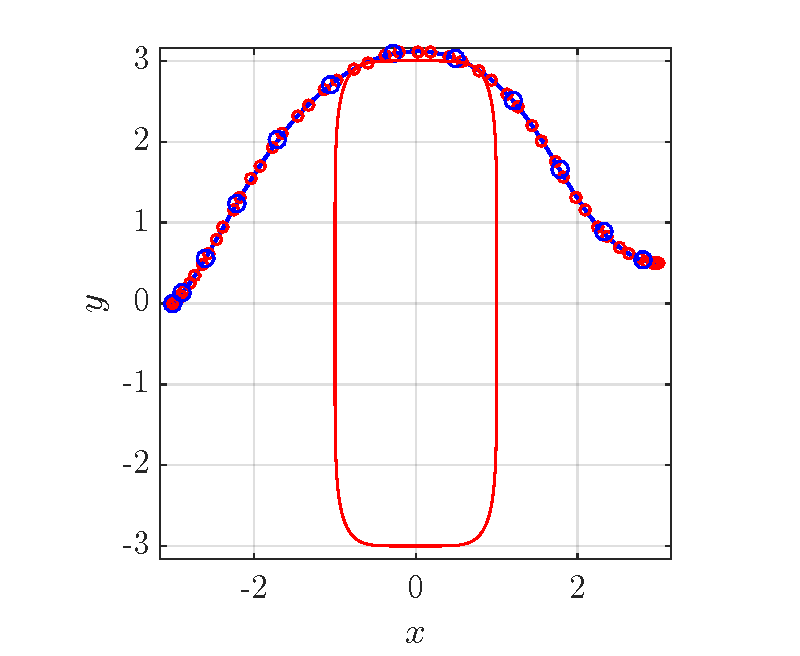
\includegraphics[width=0.33\textwidth, clip=true,trim=0.15in 0in 0.55in 0.25in]{VariationalPathPlan_Rec2}}\label{fig:VariationalPathPlan_Rec2}}
		\subfloat[$\halfL_o=(1,5)$ and $p=2$]
    {{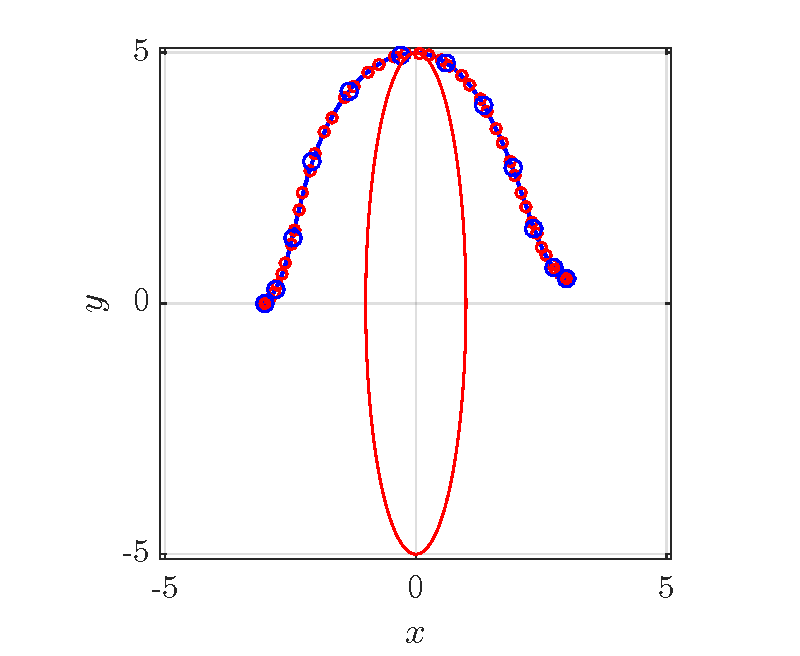
\includegraphics[width=0.36\textwidth, clip=true,trim=0.15in 0in 0.55in 0.25in]{VariationalPathPlan_Rec3}}\label{fig:VariationalPathPlan_Rec3}}
\caption{Solution to the BVP}
\label{fig:simulation}
\end{figure*}
In this examples, $T=1$ is chosen, and $50$ points are samples with the Gaussian-Legendre quadrature approximation to each node points and the points in between the node points. 12 piecewise B-splines with order 7 are used to approximated. The error to the all the constraints (boundary values and the dynamics and nonholonomic constraint) are less than $10^{-7}$. The computation time are less than 6 seconds.

 
\section{Open questions}
 
\subsection{Free final time problem with bounded velocities}

Since the above solution to the BVP generates the nominal trajectory for a given $T>0$. We can denote such solution as $g_T: [0,T]\to SE(2)$. Observe that the solution $g_T$ is continuously differentiable over the compact interval $[0,T]$, and so there exists $B:=[B_1, B_2]>0$ such that $\dot{x}^2(t)+\dot{y}^2(t) \leq B_1$, and $|\dot{\theta}(t)|\leq B_2$ for all $t\in[0,T]$. 

\begin{prob}[Existence of $T$ over fixed $B$]
\label{prbo:existence_T}
 Given $B_1>0$ and $B_2>0$, does there exist $T>0$ such that the solution $g_T$ of the ODE, (\ref{eqn:dyn1}-\ref{eqn:dyn3}), with boundary value condition (\ref{eqn:bv_initial_config}-\ref{eqn:bv_final_speed}) and nonholonomic constraint (\ref{eqn:nonholonomic}) satisfies
\begin{eqnarray}
\label{eqn:bound_linear}
\dot{x}^2(t)+\dot{y}^2(t)\leq B_1
\\
\label{eqn:bound_angular}
|\dot{\theta}(t)|\leq B_2
\end{eqnarray}
for all $t\in[0,T]$.
\end{prob}

\subsection{Minimum time problem with bounded velocities}
Suppose that Problem~\ref{prbo:existence_T} has a solution for any given $B_1, B_2>0$ pair, find the minimum $T$ which achieve the goal. 

\begin{prob}[Minimum $T$ given the bound for linear and angular speed]
\label{prbo:minimum_T}
Given $B_1>0$ and $B_2>0$, find the minimum $T$ such that the solution $g_T$ satisfies (\ref{eqn:bound_linear}) and (\ref{eqn:bound_angular}). 
\begin{equation*} 
\min_{T} T
\end{equation*}
subject to 
\begin{eqnarray*}
(\ref{eqn:dyn1}-\ref{eqn:dyn3}) &:&\text{dynamic constraints}
\\
(\ref{eqn:bv_initial_config}-\ref{eqn:bv_final_speed}) &:&\text{boundary values}
\\
(\ref{eqn:nonholonomic}) &:&\text{nonholonomic constraint}
\\
(\ref{eqn:bound_linear}-\ref{eqn:bound_angular}) &:&\text{bounds for linear and angular velocity}
\end{eqnarray*}
\end{prob}

If the optimal solution exist, then it could be a suboptimal solution to the original minimum time problem but we may have a \emph{smooth} solution as oppose to the bang bang type of solution for velocity control. 

\subsection{Kinematic control} 

What would be the control for the unicycle in this case? Can we derive a state feedback controller? 
\subsection{Non point-mass unicycle} 
How would we incorporate the actual body of the unicycle (asymmetric body- not the circular one). In the original obstacle potential only demonstrates the collision avoidance to the trajectory. However, this trajectory could be a path for a center of mass of actual non point-mass robot. How do we handle the actual geometry of the robot? 

%%%%%%%%%%%%%%%%%%%%%%%%%%%%%%%%%%%%%%%%%%%%%%%%%%%%%%%%%%%%%%%%%%%%%%%%%%%%%%%%
%
% Conclusion
%
%%%%%%%%%%%%%%%%%%%%%%%%%%%%%%%%%%%%%%%%%%%%%%%%%%%%%%%%%%%%%%%%%%%%%%%%%%%%%%%%

%\section{CONCLUSIONS}
%\label{sec_con}



\addtolength{\textheight}{-12cm}   % This command serves to balance the column lengths
                                  % on the last page of the document manually. It shortens
                                  % the textheight of the last page by a suitable amount.
                                  % This command does not take effect until the next page
                                  % so it should come on the page before the last. Make
                                  % sure that you do not shorten the textheight too much.

%%%%%%%%%%%%%%%%%%%%%%%%%%%%%%%%%%%%%%%%%%%%%%%%%%%%%%%%%%%%%%%%%%%%%%%%%%%%%%%%



%%%%%%%%%%%%%%%%%%%%%%%%%%%%%%%%%%%%%%%%%%%%%%%%%%%%%%%%%%%%%%%%%%%%%%%%%%%%%%%%
%
% ACKNOWLEDGMENT
%
%%%%%%%%%%%%%%%%%%%%%%%%%%%%%%%%%%%%%%%%%%%%%%%%%%%%%%%%%%%%%%%%%%%%%%%%%%%%%%%
%\section*{ACKNOWLEDGMENT}
%The authors especially appreciate the valuable discussion with
%Dr.~Anthony Yezzi and Dr.~Sung Ha Kang.


%%%%%%%%%%%%%%%%%%%%%%%%%%%%%%%%%%%%%%%%%%%%%%%%%%%%%%%%%%%%%%%%%%%%%%%%%%%%%%%%
%
% Reference
%
%%%%%%%%%%%%%%%%%%%%%%%%%%%%%%%%%%%%%%%%%%%%%%%%%%%%%%%%%%%%%%%%%%%%%%%%%%%%%%%%

\bibliographystyle{IEEEtran} % use IEEEtran.bst style
\bibliography{VariationalPathPlanLp}


\end{document}
